\chapter{Orthonormal Bases and Complements}\label{orthonormalbases}

You may have noticed that we have only rarely used the dot product. That is because many of the
results we have obtained do not require a preferred notion of lengths of vectors. Once a dot or inner product
is available, lengths of and angles between vectors can be measured--very powerful machinery and results are available
in this case.

\section{Properties of the Standard Basis}

The standard notion of the length of a vector $x=(x_1,x_2,\ldots,x_n)$ $\in$ ${\mathbb R}^n$ is 
\[||x||=\sqrt{x\dotprod x}=\sqrt{(x_1)^2+(x_2)^2+\cdots(x_n)^2}\, .\]
The canonical/standard basis in ${\mathbb R}^n$
\[
e_1=\colvec{1\\0\\ \vdots \\ 0}, \phantom{X}
e_2=\colvec{0\\1\\ \vdots \\ 0}, \phantom{X} \ldots, 
\phantom{X} e_n=\colvec{0\\0\\ \vdots \\ 1}\, ,
\]
has many useful properties with respect to the dot product and lengths.
\begin{itemize}
\item Each of the standard basis vectors has unit length;
\[
\|e_i\|=\sqrt{e_i\dotprod e_i}=\sqrt{e_i^Te_i}=1\, .\]
\item The standard basis vectors are \emph{orthogonal}\index{Orthogonal}\label{orthogonal} (in other words, at right angles or perpendicular); 
\[
e_i\dotprod e_j = e_i^Te_j=0 \text{ when } i\neq j
\]
\end{itemize}
This is summarized by
\[
e_i^Te_j=\delta_{ij}=\left\{ \begin{array}{cc}
1 & \qquad i=j \\
0 & \qquad i\neq j \\
\end{array}\right. ,
\]
where $\delta_{ij}$ is the \emph{Kronecker delta}\index{Kronecker delta}.  Notice that the Kronecker delta gives the entries of the identity matrix.

Given column vectors $v$ and $w$, we have seen that the dot product $v\dotprod w$ is the same as the matrix multiplication $v^Tw$.  This is an \emph{inner product}\index{Inner product} on~$\Re^n$.  We can also form the \emph{outer product}\index{Outer product} $vw^T$, which gives a square matrix.
The outer product on the standard basis vectors is interesting.  Set 
\begin{align*}
\Pi_1 &= e_1e_1^T \\
  &= \colvec{1\\0\\ \vdots \\ 0} \rowvec{1&0& \cdots & 0}\\
  &= \begin{pmatrix}
      1 & 0 & \cdots & 0 \\
      0 & 0 & \cdots & 0 \\
      \vdots & & & \vdots \\
      0 & 0 &\cdots & 0
      \end{pmatrix}\\
&\vdots \\
\Pi_n &= e_n e_n^T \\
  &= \colvec{0\\0\\ \vdots \\ 1} \rowvec{0&0& \cdots & 1}\\
  &= \begin{pmatrix}
      0 & 0 & \cdots & 0 \\
      0 & 0 & \cdots & 0 \\
      \vdots & & & \vdots \\
      0 & 0 &\cdots & 1
      \end{pmatrix}
\end{align*}
In short, $\Pi_i$ is the diagonal square matrix with a $1$ in the $i$th diagonal position and zeros everywhere else\footnote{This is reminiscent of an older notation, where vectors are written in juxtaposition.  This is called a \href{http://en.wikipedia.org/wiki/Dyadic_tensor}{``dyadic tensor''}\index{Dyad}, and is still used in some applications. }.

Notice that 
$\Pi_i\Pi_j=e_ie_i^Te_je_j^T=e_i\delta_{ij}e_j^T$.  Then:
\[
\Pi_i\Pi_j = \left\{ \begin{array}{cc}
\Pi_i & \qquad i=j \\
0 & \qquad i\neq j \\
\end{array}\right. .
\]
Moreover, for a diagonal matrix $D$ with diagonal entries $\lambda_1,\ldots, \lambda_n$, we can write
\[
D= \lambda_1\Pi_1 + \cdots + \lambda_n\Pi_n.
\]

\section{Orthogonal and Orthonormal Bases}

There are many other bases that  behave in the same way as the standard basis.  As such, we will study:
\begin{itemize}
\item \emph{Orthogonal bases}\index{Orthogonal basis} $\{v_1, \ldots, v_n \}$:
\[
v_i\dotprod v_j=0 \text{ if } i\neq j\, .
\]
In other words, all vectors in the basis are perpendicular.

\item \emph{Orthonormal bases}\index{Orthonormal basis} $\{u_1, \ldots, u_n \}$:
\[
u_i\dotprod u_j = \delta_{ij}.
\]
In addition to being orthogonal, each vector has unit length.
\end{itemize}

Suppose $T=\{u_1, \ldots, u_n \}$ is an orthonormal basis for $\Re^n$.  Because $T$ is a basis, we can write any vector $v$ uniquely as a linear combination of the vectors in $T$;
\[
v=c^1u_1+\cdots c^nu_n.
\]
Since $T$ is orthonormal, there is a very easy way to find the coefficients of this linear combination.  By taking the dot product of $v$ with any of the vectors in $T$, we get
\begin{align*}
v\dotprod u_i &= c^1u_1\dotprod u_i + \cdots + c^iu_i\dotprod u_i + \cdots + c^nu_n\dotprod u_i \\
& = c^1\cdot 0 + \cdots + c^i\cdot 1 + \cdots + c^n\cdot 0 \\
& = c^i, \\[1mm]
\Rightarrow\, c^i &= v\dotprod u_i \\[1mm]
\Rightarrow\  v &= (v\dotprod u_1) u_1 + \cdots + (v\dotprod u_n)u_n\\
&= \sum_i (v\dotprod u_i)u_i\, .
\end{align*}

This proves the following theorem.
\begin{theorem}
For an orthonormal basis $\{u_1, \ldots, u_n \}$, any vector $v$ can be expressed as
\[
v =\sum_i (v\dotprod u_i)u_i.
\]
\end{theorem}

\Reading{OrthonormalBases}{1}
%\begin{center}\href{\webworkurl ReadingHomework21/1/}{Reading homework: problem \ref{orthonormalbases}.1}\end{center}

\Videoscriptlink{orthonormal_bases_sin_cos.mp4}{All orthonormal bases for $\mathbb{R}^2$}{scripts_orthonormal_bases_sin_cos}

\subsection{Orthonormal Bases and Dot Products}

To calculate lengths of, and angles between vectors in ${\mathbb R}^n$ we most commonly use the dot product:
\[
\colvec{v^1\\\mc \vdots \\ v^n}\cdot \colvec{w^1\\\mc \vdots \\ w^n}:=v^1 w^1 + \cdots + v^n w^n\, .
\] 
When dealing with more general vector spaces
the dot product makes no sense, and one must instead choose an appropriate inner product. By ``appropriate'', we mean an inner product well-suited to the problem one is trying to solve. If the vector space $V$ under study has an orthonormal basis $O=(u_1,\ldots, u_n)$ meaning 
\[
\langle u_i,u_j\rangle=\delta_{ij}\, ,
\]
where $\langle\cdot,\cdot\rangle$ is the inner product, you might ask whether this can be related to a dot product? The answer to this question is yes and rather easy to understand:

Given an orthonormal basis, the information of two vectors $v$ and $v'$ in~$V$ can be encoded in column vectors
\begin{align*}
v&= \langle v,u_1\rangle u_1 + \cdots +\langle v,u_n\rangle u_n\, =
\hspace{.3mm}(u_1,\ldots, u_n) \colvec{\langle v,u_1\rangle\\\mc\vdots\\\langle v,u_n\rangle}\hspace{.4mm}=\colvec{\langle v,u_1\rangle\\\mc\vdots\\\langle v,u_n\rangle}_{\! O}\, ,\\[2mm]
v'&=\langle v',u_1\rangle u_1 + \cdots+ \langle v',u_n\rangle u_n=(u_1,\ldots, u_n)\hspace{-.2mm} \colvec{\langle v',u_1\rangle\\\mc\vdots\\\langle v',u_n\rangle}\hspace{-.2mm}=
\hspace{-.2mm}\colvec{\langle v',u_1\rangle\\\mc\vdots\\\langle v',u_n\rangle}_{\! O}\, .
\end{align*}
The dot product of these two column vectors is
\[
\colvec{\langle v,u_1\rangle\\\mc\vdots\\\langle v,u_n\rangle}\cdot \colvec{\langle v',u_1\rangle\\\mc\vdots\\\langle v',u_n\rangle}=
\langle v,u_1\rangle\langle v',u_1\rangle+\cdots+\langle v,u_n\rangle\langle v,'u_n\rangle\, .
\]
This agrees exactly with the inner product of $v$ and $v'$ because
\begin{align*}
\langle v,v'\rangle&= \big\langle
\langle v,u_1\rangle u_1 + \cdots +\langle v,u_n\rangle u_n,\langle v',u_1\rangle u_1 + \cdots+ \langle v',u_n\rangle u_n
\big\rangle
\\[1mm]
&=
\langle v,u_1\rangle \langle v',u_1\rangle \langle u_1,u_1\rangle + \langle v,u_2\rangle \langle v',u_1\rangle \langle u_2,u_1\rangle+\cdots \\
&\cdots+
\langle v,u_{n-1}\rangle \langle v',u_n\rangle \langle u_{n-1},u_n\rangle + \langle v,u_n\rangle \langle v',u_n\rangle \langle u_n,u_n\rangle\\[1mm]
&=
\langle v,u_1\rangle\langle v',u_1\rangle+\cdots+\langle v,u_n\rangle\langle v',u_n\rangle\, .
\end{align*}
The above computation looks a little daunting, but only the linearity property of inner products and the fact that $\langle u_i,u_j\rangle$ can  equal either zero or one was used.
Because inner products become dot products once one uses an orthonormal basis, we will quite often use the dot product notation in situations where one really should write an inner product. Conversely, dot product computations can always be rewritten in terms of an inner product, if needed.

\begin{example}
Consider the space of polynomials given by $V=\span\{1,x\}$ with inner product $\langle p,p'\rangle=\int_0^1  p(x) p'(x)dx $. An obvious basis to use is $B=(1,x)$ 
but it is not hard to check that this is not orthonormal, instead we take \[O=\Big(1,{2\sqrt{3}}\, \big(x-\frac12\big)\Big)\, .\]
This is an orthonormal basis  since,for example:
\[
\Big\langle{2\sqrt{3}}\big(x-\frac12\big),1\Big\rangle
={2\sqrt{3}}\int_0^1 \big(x-\frac12\big)dx=0\, ,\]
and 
\[
\Big\langle x-\frac12,x-\frac12\Big\rangle=
\int_0^1 \big(x-\frac12\big)^2dx=\frac{1}{12}=\Big(\frac{1}{2\sqrt{3}}\Big)^2\, .
\]
An arbitrary vector $v=a+b x$ is given in terms of the orthonormal basis $O$ by
\[
v=(a+\frac b2).1 + b \big(x-\frac12\big) =\Big(1,{2\sqrt{3}}\, \big(x-\frac12\big)\Big)
\colvec{a+\frac b2\\[2mm] \mc{\frac{b}{2\sqrt{3}}}}=\colvec{a+\frac b2\\[2mm] \mc{\frac{b}{2\sqrt{3}}}}_{\! O}\, .
\]
Hence   we can predict the inner product of $a+bx$ and $a'+b'x$ using the dot product:
\[\colvec{a+\frac b2\\[2mm] \mc{\frac{b}{2\sqrt{3}}}}\cdot \colvec{a'+\frac {b'}2\\[2mm] \mc{\frac{b'}{2\sqrt{3}}}}
=\Big(a+\frac b2\Big) \Big(a'+\frac {b'}2\Big) + \frac{b b'}{12}=aa'+\frac12\, (ab'+a'b) + \frac13\, bb'\, . \]
Indeed
\[
\langle a+bx,a'+b'x\rangle = \int_0^1 (a+bx)(a'+b'x)dx=aa'+\frac12\, (ab'+a'b) + \frac13\, bb'\, .
\]
\end{example}

\section{Relating Orthonormal Bases}

Suppose $T=\{u_1, \ldots, u_n \}$ and $R=\{w_1, \ldots, w_n \}$ are two orthonormal bases for $\Re^n$.  Then\\[3mm]
\begin{align*}
w_1 &= (w_1\dotprod u_1) u_1 + \cdots + (w_1\dotprod u_n)u_n\\
 & \vdots \\
w_n &= (w_n\dotprod u_1) u_1 + \cdots + (w_n\dotprod u_n)u_n\\
\Rightarrow w_i &= \sum_j u_j(u_j\dotprod w_i)
\end{align*}
Thus the matrix for the change of basis from $T$ to $R$ is given by 
\[
P = (p^j_i) = (u_j\dotprod w_i).
\]
We would like to calculate the product $PP^T$. For that, we first develop a dirty trick for products of dot products:
\[
(u\dotprod v)(w\dotprod z)=(u^T v) (w^T z) = u^T (v w^T) z\, . 
\]
The object $v w^T$ is the square matrix made from the outer product of $v$ and~$w$. 
Now we are ready to compute the components of the matrix product $PP^T$.
\begin{align*}
\sum_i(u_j\dotprod w_i)(w_i\dotprod u_k)&=
 \sum_i(u_j^T w_i) (w_i^T u_k)\\
&= u_j^T \left[\sum_i (w_i w_i^T) \right] u_k \\
&\stackrel{(*)}= u_j^T I_n u_k \\\
&= u_j^T u_k = \delta_{jk}.
\end{align*}
The equality $(*)$ is explained below.  Assuming $(*)$ holds, we have shown that $PP^T=I_n$, which implies that 
\[
P^T=P^{-1}.
\]

The equality in the line $(*)$ says that $\sum_i w_i w_i^T=I_n$.  To see this, we examine $\left(\sum_i w_i w_i^T\right)v$ for an arbitrary vector $v$.  We can find constants $c^j$ such that $v=\sum_j c^jw_j$, so that
\begin{align*}
\left(\sum_i w_i w_i^T\right)v
&= \left(\sum_i w_i w_i^T\right)\left(\sum_j c^jw_j\right) \\
&= \sum_j c^j \sum_i w_i w_i^T w_j \\
&= \sum_j c^j \sum_i w_i \delta_{ij} \\
&= \sum_j c^j w_j \text{ since all terms with $i\neq j$ vanish}\\
&=v.
\end{align*}
Thus, as a linear transformation, $\sum_i w_i w_i^T=I_n$ fixes every vector, and thus must be the identity $I_n$.

\begin{definition}
A matrix $P$ is {\bfseries orthogonal}\index{Orthogonal matrix} if $P^{-1}=P^T$.
\end{definition}

Then to summarize,
\begin{theorem}
A change of basis matrix $P$ relating two orthonormal bases is an orthogonal matrix.  \textit{I.e.},
\Shabox{1}{$
P^{-1}=P^T\, .
$}
\end{theorem}

\Reading{OrthonormalBases}{2}
%\begin{center}\href{\webworkurl ReadingHomework21/2/}{Reading homework: problem \ref{orthonormalbases}.2}\end{center}

\begin{example}
Consider $\Re^3$ with the ordered orthonormal basis 
\[
S=\left( u_1,u_2,u_3\right) 
=\left(
\colvec{\frac{2}{\sqrt{6}}\\[1mm] \frac{1}{\sqrt{6}}\\[1mm] \frac{-1}{\sqrt{6}}},
\colvec{0\\[1mm] \frac{1}{\sqrt{2}}\\[1mm] \frac{1}{\sqrt{2}}},
\colvec{\frac{1}{\sqrt{3}}\\[1mm] \frac{-1}{\sqrt{3}}\\[1mm] \frac{1}{\sqrt{3}}}
\right).
\]
Let $E$ be the standard basis $(e_1,e_2,e_3 )$.  Since we are changing from the standard basis to a new basis, then the columns of the change of basis matrix are exactly the  new basis vectors.  Then the change of basis matrix from $E$ to $S$ is given by
\begin{align*}
P=(P^j_i)=(e_j\cdot u_i)
&=
\begin{pmatrix}
e_1\dotprod u_1 & e_1\dotprod u_2 & e_1\dotprod u_3 \\
e_2\dotprod u_1 & e_2\dotprod u_2 & e_2\dotprod u_3 \\
e_3\dotprod u_1 & e_3\dotprod u_2 & e_3\dotprod u_3
\end{pmatrix} \\
= \begin{pmatrix}
u_1 & u_2 & u_3
\end{pmatrix} 
&=
\begin{pmatrix}
\frac{2}{\sqrt{6}} & 0 & \frac{1}{\sqrt{3}} \\[1mm]
\frac{1}{\sqrt{6}}& \frac{1}{\sqrt{2}}&\frac{-1}{\sqrt{3}}\\[1mm]
\frac{-1}{\sqrt{6}}& \frac{1}{\sqrt{2}}&\frac{1}{\sqrt{3}}
\end{pmatrix}.
\end{align*}

From our theorem, we observe that
\begin{align*}
P^{-1}=P^T
&= \colvec{u_1^T\\u_2^T\\u_3^T} \\
&= \begin{pmatrix}
\frac{2}{\sqrt{6}}& \frac{1}{\sqrt{6}}& \frac{-1}{\sqrt{6}}\\[1mm]
0 & \frac{1}{\sqrt{2}}&\frac{1}{\sqrt{2}} \\[1mm]
\frac{1}{\sqrt{3}}& \frac{-1}{\sqrt{3}}&\frac{1}{\sqrt{3}}
\end{pmatrix}.
\end{align*}

We can check that $P^TP=I$ by a lengthy computation, or more simply, notice that
\begin{align*}
(P^TP)%_{ij}
&= \colvec{u_1^T\\u_2^T\\u_3^T} \rowvec{u_1 & u_2& u_3} \\
&= \begin{pmatrix}1&0&0\\0&1&0\\0&0&1\end{pmatrix}.
\end{align*}
Above we are using orthonormality of the $u_i$ and the fact that matrix multiplication amounts to taking dot products between rows and columns.
It is also very \hypertarget{basisorthog}{important to realize that the columns of an {\itshape orthogonal} matrix are made
from an {\itshape orthonormal} set of vectors}.
\end{example}

\begin{remark}[Orthonormal Change of Basis and Diagonal Matrices.]
Suppose $D$ is a diagonal matrix  and we are able to use an orthogonal matrix $P$ to change to a new basis.  Then the matrix $M$ of $D$ in the new basis is:
\[
M = PDP^{-1} = PDP^T.
\]
Now we calculate the transpose of $M$.
\begin{align*}
M^T
&= (PDP^T)^T\\
&= (P^T)^TD^TP^T \\
&= PDP^T\\
&= M
\end{align*}
The matrix $M=PDP^T$ is symmetric!
\end{remark}


%\section*{References}
%Hefferon, Chapter Three, Section V: Change of Basis
%\\
%Beezer, Chapter V, Section O, Subsection N
%\\
%Beezer, Chapter VS, Section B, Subsection OBC
%\\
%Wikipedia:
%\begin{itemize}
%\item \href{http://en.wikipedia.org/wiki/Orthogonal_matrix}{Orthogonal Matrix}
%\item \href{http://en.wikipedia.org/wiki/Diagonalizable_matrix}{Diagonalizable Matrix}
%\item \href{http://en.wikipedia.org/wiki/Similar_matrix}{Similar Matrix}
%\end{itemize}

%\section{Review Problems}
%



\begin{enumerate}
\item \label{det33} Let $M=\begin{pmatrix}
m^1_1 & m^1_2 & m^1_3\\
m^2_1 & m^2_2 & m^2_3\\
m^3_1 & m^3_2 & m^3_3\\
\end{pmatrix}$.  Use row operations to put $M$ into \emph{row echelon form}.  For simplicity, assume that $m_1^1\neq 0 \neq m^1_1m^2_2-m^2_1m^1_2$.

Prove that $M$ is non-singular if and only if:
\[
m^1_1m^2_2m^3_3 
- m^1_1m^2_3m^3_2 
+ m^1_2m^2_3m^3_1 
- m^1_2m^2_1m^3_3 
+ m^1_3m^2_1m^3_2
- m^1_3m^2_2m^3_1
\neq 0
\]

\phantomnewpage

\item 
\begin{enumerate}
\item What does the matrix $E^1_2=\begin{pmatrix}
0 & 1 \\
1 & 0
\end{pmatrix}$ do to $M=\begin{pmatrix}
a & b \\
d & c
\end{pmatrix}$ under left multiplication?  What about right multiplication?
\item Find elementary matrices $R^1(\lambda)$ and $R^2(\lambda)$ that respectively multiply rows $1$ and $2$ of $M$ by $\lambda$ but otherwise leave $M$ the same under left multiplication.
\item Find a matrix $S^1_2(\lambda)$ that adds a multiple $\lambda$ of row $2$ to row $1$ under left multiplication.
\end{enumerate}

\phantomnewpage

\item Let $M$ be a matrix and $S^i_jM$ the same matrix with rows \(i\) and \(j\) switched.  Explain every line of the 
\hyperlink{rowswap}{series of equations} proving that $\det M = -\det (S^i_jM)$.

\phantomnewpage

%\item \label{prob_inversion_number} This problem is a ``hands-on'' look at why \hyperlink{permutation_parity}{the property} describing the parity of permutations is true.
%
%\hypertarget{inversion_number}{The \emph{inversion number}}\index{Permutation!Inversion number} of a permutation $\sigma$ is the number of pairs $i<j$ such that $\sigma(i)>\sigma(j)$; it's the number of ``numbers that appear left of smaller numbers'' in the permutation.  For example, for the permutation $\rho = [4,2,3,1]$, the inversion number is $5$. The number $4$ comes before $2,3,$ and $1$, and $2$ and $3$ both come before $1$.
%
%Given a permutation $\sigma$, we can make a new permutation $\tau_{i,j} \sigma$ by exchanging the $i$th and $j$th entries of $\sigma$.
%
%\begin{enumerate}
%\item What is the inversion number of the permutation \(\mu=[1,2,4,3]\) that exchanges 4 and 3 and leaves everything else alone? Is it an even or an odd permutation?
%
%\item What is the inversion number of the permutation \(\rho=[4,2,3,1]\) that exchanges 1 and 4 and leaves everything else alone? Is it an even or an odd permutation?
%
%\item What is the inversion number of the permutation \(\tau_{1,3} \mu\)? Compare the parity\footnote{The \emph{parity} of an integer refers to whether the integer is even or odd. Here the parity of a permutation $\mu$ refers to the parity of its inversion number.} of \(\mu\) to the parity of \(\tau_{1,3} \mu.\)
%
%\item What is the inversion number of the permutation \(\tau_{2,4} \rho\)? Compare the parity of \(\rho\) to the parity of \(\tau_{2,4} \rho.\)
%
%\item What is the inversion number of the permutation \(\tau_{3,4} \rho\)? Compare the parity of \(\rho\) to the parity of \(\tau_{3,4} \rho.\)
%\end{enumerate}
%
%\videoscriptlink{elementary_matrices_determinant_hint.mp4}{Problem~\ref{prob_inversion_number} hints}{scripts_elementary_matrices_determinants_hint}

\phantomnewpage

%\item \label{problem_permutation} (Extra credit) Here we will examine a (very) small set of the general properties about permutations and their applications. In particular, we will show that one way to compute the sign of a permutation is by finding the \hyperlink{inversion_number}{inversion number} $N$ of $\sigma$ and we have
%\[
%\sgn(\sigma) = (-1)^N.
%\]
%
%For this problem, let $\mu = [1,2,4,3]$.
%
%\begin{enumerate}
%\item Show that every permutation $\sigma$ can be sorted by only taking simple (adjacent) transpositions\index{Permutation!Simple transposition} $s_i$ where $s_i$ interchanges the numbers in position $i$ and $i+1$ of a permutation $\sigma$ (in our other notation $s_i = \tau_{i,i+1}$). For example $s_2 \mu = [1, 4, 2, 3]$, and to sort $\mu$ we have $s_3 \mu = [1, 2, 3, 4]$.
%
%\item \label{prob_part_relations} We can compose simple transpositions together to represent a permutation (note that the sequence of compositions is not unique), and these are associative, we have an identity (the trivial permutation where the list is in order or we do nothing on our list), and we have an inverse since it is clear that $s_i s_i \sigma = \sigma$. Thus permutations of $[n]$ under composition are an example of a \hyperref[groups]{group}. However note that not all simple transpositions commute with each other since
%\begin{align*}
%s_1 s_2 [1, 2, 3] & = s_1 [1, 3, 2] = [3, 1, 2]
%\\ s_2 s_1 [1, 2, 3] & = s_2 [2, 1, 3] = [2, 3, 1]
%\end{align*}
%(you will prove here when simple transpositions commute). When we consider our initial permutation to be the trivial permutation $e = [1, 2, \dotsc, n]$, we do not write it; for example $s_i \equiv s_i e$ and $\mu = s_3 \equiv s_3 e$. This is analogous to not writing 1 when multiplying. Show that $s_i s_i = e$ (in shorthand $s_i^2 = e$), $s_{i+1} s_i s_{i+1} = s_i s_{i+1} s_i$ for all $i$, and $s_i$ and $s_j$ commute for all $|i - j| \geq 2$.
%
%\item Show that every way of expressing $\sigma$ can be obtained from using the relations proved in part~\ref{prob_part_relations}. In other words, show that for any expression $w$ of simple transpositions representing the trivial permutation $e$, using the proved relations.
%
%\emph{Hint: Use induction on $n$. For the induction step, follow the path of the $(n+1)$-th strand by looking at $s_n s_{n-1} \cdots s_k s_{k\pm1} \cdots s_n$ and argue why you can write this as a subexpression for any expression of $e$. Consider using diagrams of these paths to help.}
%
%\item The simple transpositions \hyperlink{action}{acts on} an $n$-dimensional vector space $V$ by $s_i v = E^i_{i+1} v$ (where $E^i_j$ is \hyperlink{elem_matrix_row_swap}{an elementary matrix}) for all vectors $v \in V$. Therefore we can just represent a permutation $\sigma$ as the matrix $M_{\sigma}$\footnote{Often people will just use $\sigma$ for the matrix when the context is clear.}, and we have $\det(M_{s_i}) = \det(E^i_{i+1}) = -1$. Thus prove that $\det(M_{\sigma}) = (-1)^N$ where $N$ is a number of simple transpositions needed to represent $\sigma$ as a permutation. You can assume that $M_{s_i s_j} = M_{s_i} M_{s_j}$ (it is not hard to prove) and that $\det(A B) = \det(A) \det(B)$ \hyperref[detmultiplicative]{from Chapter~\ref*{elementarydeterminantsII}}.
%
%\emph{Hint: You to make sure $\det(M_{\sigma})$ is well-defined since there are infinite ways to represent $\sigma$ as simple transpositions.}
%
%\item Show that $s_{i+1} s_i s_{i+1} = \tau_{i, i+2}$, and so give one way of writing $\tau_{i, j}$ in terms of simple transpositions? Is $\tau_{i,j}$ an even or an odd permutation? What is $\det(M_{\tau_{i,j}})$? What is the inversion number of $\tau_{i,j}$?
%
%\item The minimal number of simple transpositions needed to express $\sigma$ is called the \emph{length}\index{Permutation!Length} of $\sigma$; for example the length of $\mu$ is 1 since $\mu = s_3$. Show that the length of $\sigma$ is equal to the inversion number of $\sigma$.
%
%\emph{Hint: Find an procedure which gives you a new permutation $\sigma^{\prime}$ where $\sigma = s_i \sigma^{\prime}$ for some $i$ and the inversion number for $\sigma^{\prime}$ is 1 less than the inversion number for $\sigma$.}
%
%\item Show that $(-1)^N = \sgn(\sigma) = \det(M_{\sigma})$, where $\sigma$ is a permutation with $N$ inversions. Note that this immediately implies that $\sgn(\sigma \rho) = \sgn(\sigma) \sgn(\rho)$ for any permutations $\sigma$ and $\rho$.
%\end{enumerate}

\item Let $M'$ be the matrix obtained from $M$ by swapping two columns $i$ and $j$. Show that $\det M'=-\det M $.

\item The scalar triple product of three vectors $u,v,w$ from $\Re^3$ is $u\cdot(v\times w)$. Show that this product is the same as the determinant of the matrix whose columns are $u,v,w$ (in that order). What happens to the scalar triple product when the factors are permuted? 

\item Show that if $M$ is a $3\times 3$ matrix whose third row is a sum of multiples of the other rows ($R_3=aR_2+bR_1$) then $\det M=0$. Show that the same is true if one of the columns is a sum of multiples of the others. 

\end{enumerate}

\phantomnewpage



\section{Gram-Schmidt \& Orthogonal Complements}\label{gramschmidt}


Given a vector $v$ and some other vector $u$ not in  $\span\{v\} $ we can construct the new vector 
\Shabox{1.1}{$
v^\perp:=v-\frac{\textstyle u\cdot v}{\textstyle u\cdot u}\, u\, .
$}
\begin{center}
\hypertarget{projectionpic}{\input{vperp.pdftex_t}}
\end{center}
This new vector $v^\perp$ is orthogonal to $u$ because 
\[
u\dotprod v^\perp = u\dotprod v - \frac{u\cdot v}{u\cdot u}u\dotprod u = 0.
\]
Hence, $\{u, v^\perp\}$ is an orthogonal basis for $\spa \{u,v\}$.  When $v$ is not parallel to $u$, $v^\perp \neq 0$, and normalizing these vectors we obtain $\left\{\frac{u}{|u|}, \frac{v^\perp}{|v^\perp|} \right\}$, an orthonormal basis for the vector space $\span\{u,v\}$.

Sometimes we write $v = v^\perp + v^\parallel$ where:
\begin{align*}
v^\perp &= v-\frac{u\cdot v}{u\cdot u}\, u \\[1mm]
v^\parallel &= \phantom{v-}\frac{u\cdot v}{u\cdot u}\, u.
\end{align*}
This is called an {\bfseries orthogonal decomposition}\index{Orthogonal decomposition} because we have decomposed $v$ into a sum of orthogonal vectors.  This decomposition depends on $u$; if we change the direction of $u$ we change $v^\perp$ and $v^\parallel$.

If $u$, $v$ are linearly independent vectors in $\Re^3$, then the set $\{u, v^\perp, u\times v^\perp \}$ would be an orthogonal basis for $\Re^3$.  This set could then be normalized by dividing each vector by its length to obtain an orthonormal basis.

However, it often occurs that we are interested in vector spaces with dimension greater than $3$, and must resort to craftier means than cross products to obtain an orthogonal basis\footnote{Actually, given a set $T$ of $(n-1)$ independent vectors in $n$-space, one can define an analogue of the cross product that will produce a vector orthogonal to the span of~$T$, using a method exactly analogous to the usual computation for calculating the cross product of two vectors in $\Re^3$.  This only gets us the ``\emph{last}'' orthogonal vector, though; the Gram--Schmidt process described in this section gives a way to get a full orthogonal basis.}.
%yeah, and who is going to teach them about the Hodge star in office hours? I say nix this footnote -cherney

Given a third vector $w$, we should first check that $w$ does not lie in the 
$\spa\{ u,v\} $, \textit{i.e.}, check that $u,v$ and $w$ are linearly independent.   If it does not, we then can define
\[
w^\perp := w - \frac{u\dotprod w}{u\dotprod u}\,u - \frac{v^\perp\dotprod w}{v^\perp\dotprod v^\perp}\,v^\perp.
\]
We can check that \(u \dotprod w^\perp\) and \(v^\perp \dotprod w^\perp\) are both zero:
\begin{align*}
u \dotprod w^\perp&=u \dotprod \left(w - \frac{u\dotprod w}{u\dotprod u}\,u - \frac{v^\perp\dotprod w}{v^\perp\dotprod v^\perp}\,v^\perp \right)\\&= u\dotprod w - \frac{u \dotprod w}{u \dotprod u}u \dotprod u - \frac{v^\perp \dotprod w}{v^\perp \dotprod v^\perp} u \dotprod v^\perp \\
&=u\dotprod w-u\dotprod w-\frac{v^\perp \dotprod w}{v^\perp \dotprod v^\perp} u \dotprod v^\perp\ =\ 0
\end{align*}
since \(u\) is orthogonal to \(v^\perp\), and
\begin{align*}
v^\perp \dotprod w^\perp&=v^\perp \dotprod \left(w - \frac{u\dotprod w}{u\dotprod u}\,u - \frac{v^\perp\dotprod w}{v^\perp\dotprod v^\perp}\,v^\perp \right)\\ &=v^\perp\dotprod w - \frac{u \dotprod w}{u \dotprod u}v^\perp \dotprod u - \frac{v^\perp \dotprod w}{v^\perp \dotprod v^\perp} v^\perp \dotprod v^\perp \\
&=v^\perp\dotprod w-\frac{u \dotprod w}{u \dotprod u}v^\perp \dotprod u - v^\perp \dotprod w\ =\ 0
\end{align*}
because \(u\) is orthogonal to \(v^\perp\). Since $w^\perp$ is orthogonal to both $u$ and $v^\perp$, we have that $\{u,v^\perp,w^\perp \}$ is an orthogonal basis for $\spa \{u,v,w\}$.

\subsection{The Gram-Schmidt Procedure}
In fact, given an ordered set $(v_1, v_2, \ldots )$ of linearly independent vectors, we can define an orthogonal basis for $\spa \{v_1,v_2, \ldots \}$ consisting of the  vectors
\begin{align*}
v_1^\perp&:=v_1 \\
v_2^\perp &:= v_2 - \frac{v_1^\perp\cdot v_2}{v_1^\perp\cdot v_1^\perp}\,v_1^\perp \\
v_3^\perp &:= v_3 - \frac{v_1^\perp\cdot v_3}{v_1^\perp\cdot v_1^\perp}\,v_1^\perp - \frac{v_2^\perp\cdot v_3}{v_2^\perp\cdot v_2^\perp}\,v_2^\perp\\
&\vdots \\
v_i^\perp%&=   v_i - \sum_{j<i} \frac{v_j^\perp\cdot v_i}{v_j^\perp\cdot v_j^\perp}\,v_j^\perp \\
 &:= v_i - \frac{v_1^\perp\cdot v_i}{v_1^\perp\cdot v_1^\perp}\,v_1^\perp   
 - \frac{v_2^\perp\cdot v_i}{v_2^\perp\cdot v_2^\perp}\,v_2^\perp -\cdots
 - \frac{v_{i-1}^\perp\cdot v_i}{v_{i-1}^\perp\cdot v_{i-1}^\perp}\,v_{i-1}^\perp\\
&\vdots
\end{align*}
Notice that each $v_i^\perp$ here depends on  $v_j^\perp$ for every $j<i$.  This allows us to inductively/algorithmically build up a linearly independent, orthogonal set of vectors 
$\{v_1^\perp,v_2^\perp, \ldots \}$ 
such that 
$\spa \{v_1^\perp,v_2^\perp, \ldots \}=\spa \{v_1, v_2, \ldots \}$. 
That is, an orthogonal basis for the latter vector space. 

Note that the set of vectors you start out with needs to be ordered to uniquely specify the algorithm; changing the order of the vectors will give a different orthogonal basis. You might need to be the one to put an order on the initial set of vectors.

This algorithm is called the {\bfseries Gram--Schmidt orthogonalization procedure}\index{Gram--Schmidt orthogonalization procedure}\label{GramSchmidt}--Gram worked at a Danish insurance company over one hundred years ago, Schmidt was a student of Hilbert (the famous German mathmatician).

\begin{example}
We'll  obtain an orthogonal basis for $\Re^3$ by appling Gram-Schmidt to the linearly independent set 
$\left\{\colvec{1\\1\\1}, \colvec{1\\1\\0},\colvec{3\\1\\1} \right\}$.\\

Because he Gram-Schmidt algorithm uses the first vector from the ordered set the largest number of times, we will choose the vector with the most zeros to be the first in hopes of simplifying computations; we choose to order the set as
\[( v_1,v_2,v_3)
:= \left( \colvec{1\\1\\0}, \colvec{1\\1\\1},\colvec{3\\1\\1} \right).\]

First, we set $v_1^\perp:=v_1$.  Then
\begin{align*}
v_2^\perp&:= \rowvec{1\\1\\1} - \frac{2}{2}\rowvec{1\\1\\0} = \rowvec{0\\0\\1} \\[2mm]
v_3^\perp&:= \rowvec{3\\1\\1} - \frac{4}{2}\rowvec{1\\1\\0} - \frac{1}{1}\rowvec{0\\0\\1} = \rowvec{1\\-1\\0}. 
\end{align*}
Then the set
\[
\left\{ \rowvec{1\\1\\0},\rowvec{0\\0\\1},\rowvec{1\\-1\\0}\right\}
\]
is an orthogonal basis for $\Re^3$.  To obtain an ortho{\itshape normal} basis we simply divide each of these vectors by its length, yielding
\[
\left\{ \rowvec{\frac{1}{\sqrt2}\\[2mm]\frac{1}{\sqrt2}\\[1mm]0},\rowvec{0\\[2mm]0\\[1mm]1},\rowvec{\frac{1}{\sqrt2}\\[2mm]\frac{-1}{\sqrt2}\\[1mm]0}\right\}.
\]
\end{example}

\Videoscriptlink{gram_schimdt_and_orthogonal_complements_4by4_example.mp4}{A $4\times4$ Gram--Schmidt Example} {scripts_gram_schmidt_and_orthogonal_complements_4by4_example}

\section{$QR$ Decomposition}
In Chapter~\ref{Matrices}, Section~\ref{LUdecomp} teaches you how to solve linear systems by decomposing a matrix $M$ into 
a product of lower and upper triangular matrices
\[M=LU\, .\]
The Gram--Schmidt procedure suggests another matrix decomposition,
\[M=QR\, ,\] 
where $Q$ is an orthogonal matrix and $R$ is an upper triangular matrix. So-called QR-decompositions\index{QR decomposition}
are useful for solving linear systems, eigenvalue problems and least squares approximations. You can
easily get the idea behind the $QR$ decomposition by working through a simple example.

\begin{example}
\hypertarget{methodQR}{Find} the $QR$ decomposition of \[M=\begin{pmatrix}2&-1&1\\1&3&-2\\0&1&-2\end{pmatrix}\, .\]
What we will do is to think of the columns of $M$ as three 3-vectors and use Gram--Schmidt to
build an orthonormal basis from these that will become the columns of the orthogonal matrix $Q$.
We will use the matrix $R$ to record the steps of the Gram--Schmidt procedure in such a way
that the product $QR$ equals $M$. 

To begin with we write
\[
M=\begin{pmatrix}2&-\frac75&1\\[1mm]1&\frac{14}5&-2\\[1mm]0&1&-2\end{pmatrix}
\begin{pmatrix}1&\frac15&0\\[1mm]0&1&0\\[1mm]0&0&1\end{pmatrix}\, .
\]
In the first matrix the first two columns are  orthogonal because we simply replaced the second column of $M$ by the vector that the Gram--Schmidt
procedure produces from the first two columns of~$M$, namely
\[
\colvec{-\frac75\\[1mm]\frac{14}5\\[1mm]1}=\colvec{-1\\[1mm]3\\[1mm]1}-\frac15
\colvec{ 2 \\[1mm]1\\[1mm]0}\, .
\]
 The matrix on the right is almost the identity
matrix, save the $+\frac15$ in the second entry of the first row, whose effect upon multiplying the
two matrices precisely undoes what we we did to the second column of the first matrix. 

For the third column of $M$ we use Gram--Schmidt to deduce the third orthogonal vector
\[
\colvec{-\frac16\\[1mm]\frac13\\[1mm]-\frac76}=
\colvec{1\\[1mm]-2\\[1mm]-2}
-0
\colvec{ 2 \\[1mm]1\\[1mm]0}
-\frac{-9}{\frac{54}{5}}\colvec{-\frac75\\[1mm]\frac{14}5\\[1mm]1}\, ,
\]
and therefore, using exactly the same procedure write
\[
M=\begin{pmatrix}2&-\frac75&-\frac16\\[1mm]1&\frac{14}5&\frac13\\[1mm]0&1&-\frac76\end{pmatrix}
\begin{pmatrix}1&\frac15&0\\[1mm]0&1&-\frac56\\[1mm]0&0&1\end{pmatrix}\, .
\]
This is not quite the answer because the first matrix is now made of mutually orthogonal column vectors,
but  a {\itshape bona fide} orthogonal matrix is comprised of {\itshape orthonormal} vectors. To achieve that we divide
each column of the first matrix by its length and multiply the corresponding row of the second matrix by the same 
amount:
\[
M=\begin{pmatrix}\frac{2\sqrt{5}}{5}&-\frac{7\sqrt{30}}{90}&-\frac{\sqrt{6}}{18}\\[2mm]
\frac{\sqrt{5}}{5}&\frac{7\sqrt{30}}{45}&\frac{\sqrt{6}}{9}\\[2mm]
0&\frac{\sqrt{30}}{18}&-\frac{7\sqrt{6}}{18}\end{pmatrix}
\begin{pmatrix}\sqrt{5}&\frac{\sqrt{5}}{5}&0\\[2mm]
0&\frac{3\sqrt{30}}{5}&-\frac{\sqrt{30}}{2}\\[2mm]
0&0&\frac{\sqrt{6}}{2}\end{pmatrix}=QR\, .
\]
Geometrically what has happened here is easy to see. We started with three vectors given by the columns of $M$ and rotated them such that the first lies along the $x$-axis, the second in the $xy$-plane and the third in some other generic direction (here it happens to be in the $yz$-plane).

A nice check of the above result is to verify that entry $(i,j)$  of the matrix $R$
equals the dot product of the $i$-th column of $Q$ with the $j$-th column of $M$.
(Some people memorize this fact and use it as a recipe for computing $QR$ decompositions.)
{\itshape A good test of your own understanding is to work out why this is true!}
\end{example}


\Videoscriptlink{gram_schimdt_and_orthogonal_complements_qr_example.mp4}{Another $QR$ decomposition example}{scripts_gram_schmidt_and_orthogonal_complements_qr_example}

\section{Orthogonal Complements}

Let $U$ and $V$ be subspaces of a vector space $W$.  In \hyperref[UcapV]{Review Exercise}~\ref{UandV}, Chapter~\ref{subspacesspanning}, you are asked to show that $U\cap V$ is a subspace of $W$, and that $U\cup V$ is {\itshape not} a subspace.  However, $\spa (U\cup V)$ {\itshape is} certainly a subspace, since the span of \emph{any} subset of a vector space is a subspace.
Notice that all elements of $\spa (U\cup V)$ take the form $u+v$ with $u\in U$ and $v\in V$.  We call the subspace 
\Shabox{1}{$
U+V:=\spa (U\cup V) = \{u+v ~| ~u\in U, v\in V \}$}
the \emph{sum}\index{Sum of vectors spaces} of $U$ and $V$.  Here, we are not adding vectors, but vector spaces to produce a new vector space.
\begin{example}
\[
\spa\left\{  \colvec{1\\1\\0\\0},  \colvec{0\\1\\1\\0} \right \} 
+ \spa\left\{  \colvec{0\\1\\1\\0},  \colvec{0\\0\\1\\1} \right \} 
= \spa\left\{  \colvec{1\\1\\0\\0},  \colvec{0\\1\\1\\0},  \colvec{0\\0\\1\\1} \right \} .
\]
Notice that the addends have elements in common; 
$\colvec{0\\1\\1\\0}$ is in both addends. Even though both of the addends are 2-dimensional their sum is not  4-dimensional.
\end{example}


In the special case that $U$ and $V$ do not have any non-zero vectors in common, their sum is a vector space with dimension $\dim U + \dim V$. 


\begin{definition}
If  $U$ and $V$ are subspaces of a vector space $W$ such that 
$U~\cap~V=~\{0_W\}\, $
then the vector space
\[
U \oplus V := \spa (U\cup V)= \{u+v ~|~ u\in U, v\in V \}
\]
is the {\bfseries direct sum}\index{Direct sum} of $U$ and $V$.
\end{definition}

\begin{remark}

$\phantom{JUNK HERE}$\\[-8mm]

\begin{itemize}
\item When $U\cap V= \{0_W\}$, $U+V=U\oplus V.$ 
\item When $U\cap V \neq \{0_W\}$, $U+V \neq U\oplus V$.
\end{itemize}
\end{remark}

\noindent This distinction is important because the direct sum has a very nice property:

\begin{theorem}
If $w\in U\oplus V$  then 
%the expression $w=u+v$ is unique.  That is, 
there is only one way to write \(w\) as the sum of a vector in \(U\) and a vector in \(V\).  
\end{theorem}

\begin{proof}
Suppose that $u+v=u'+v'$, with $u,u'\in U$, and $v,v' \in V$.  Then we could express $0=(u-u')+(v-v')$.  Then $(u-u')=-(v-v')$.  Since $U$ and $V$ are subspaces, we have $(u-u')\in U$ and $-(v-v')\in V$.  But since these elements are equal, we also have $(u-u')\in V$.  Since $U\cap V=\{0\}$, then $(u-u')=0$.  Similarly, $(v-v')=0$. Therefore $u=u'$ and  $v=v'$, proving the theorem. 
\end{proof}

\Reading{OrthonormalBases}{3}
%\begin{center}\href{\webworkurl ReadingHomework22/1/}{Reading homework: problem \ref{gramschmidt}.1}\end{center}


\noindent Here is a sophisticated algebra question:
\begin{quote}
Given a subspace $U$ in $W$, what are the solutions to 
\[ U\oplus V =W.\]
That is, how can we write $W$ as the direct sum of $U$ and \emph{something}? 
\end{quote}
There is not a unique answer to this question as can be seen from the following picture of subspaces in $W={\mathbb R}^3$. 
\begin{center}
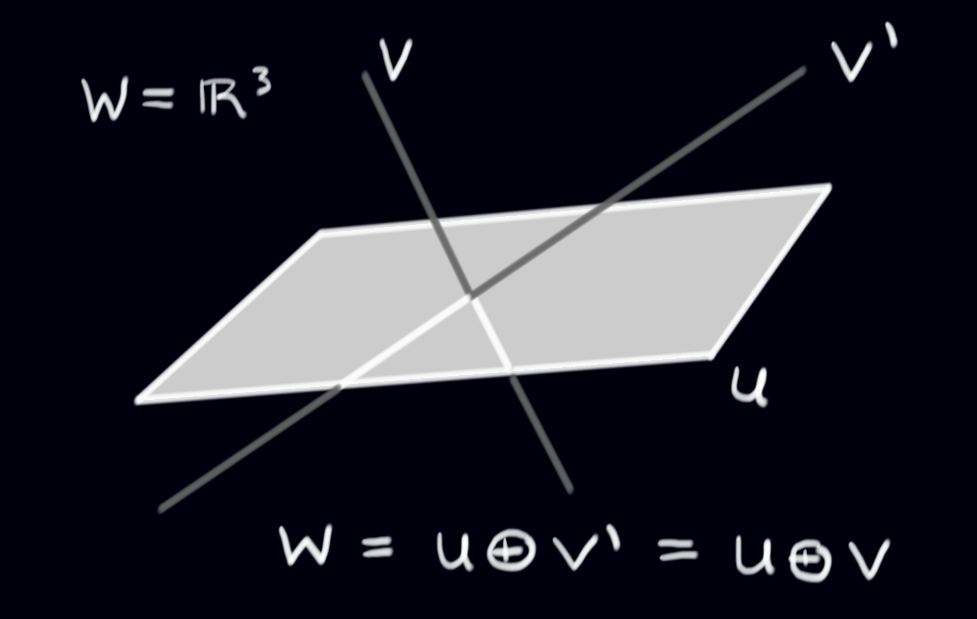
\includegraphics[scale=.25]{\gramSchmidtPath/direct_sums.jpg}
\end{center}
However, using the inner product, there is a natural candidate $U^\perp$ for this second subspace as shown below.
\begin{center}
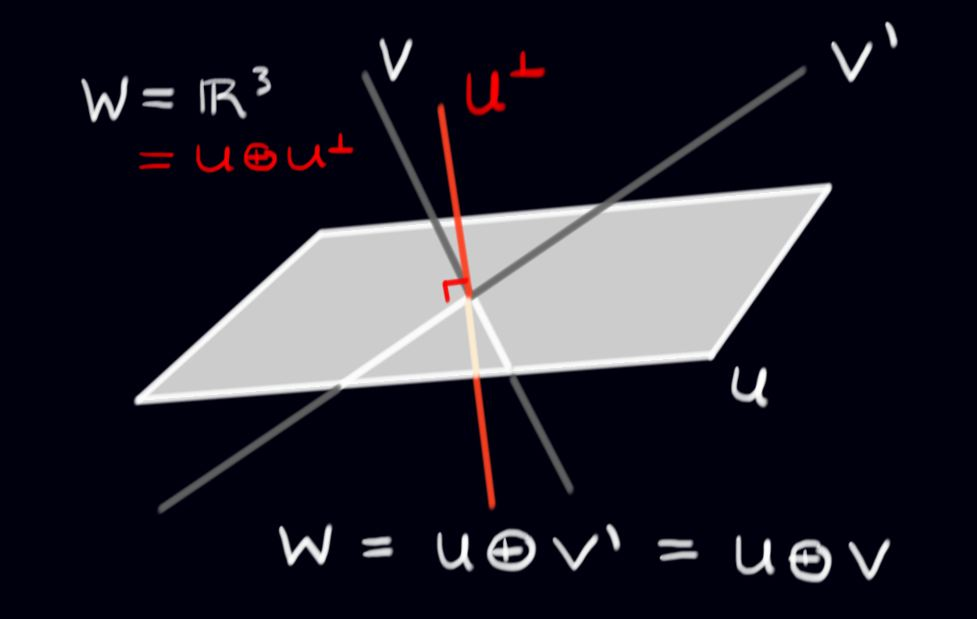
\includegraphics[scale=.25]{\gramSchmidtPath/U_perp.jpg}
\end{center}


\begin{definition}
If $U$ is a subspace of the vector space $W$ then the vector space 
\[U^\perp := \big\{w\in W \big| w\dotprod u=0 \text{ for all } u\in U\big\}\, \]
is the {\bfseries orthogonal complement}\index{Orthogonal complement} of $U$ in $W$. 
\end{definition}


\begin{remark}
The symbols ``$U^\perp$" are often read as ``$U$-perp''.  This is the set of all vectors in $W$ orthogonal to \emph{every} vector in $U$. 
Notice also that in the above definition we have implicitly assumed that the inner product is the dot product. For a general \hyperlink{inner_product}{inner product}, the  
above definition would read $U^\perp := \big\{w\in W \big|\,  \langle w,u\rangle=0 \text{~for~all~}u\in U\big\}\, $.
\end{remark}
Possibly by now you are feeling overwhelmed, it may help to watch this quick overview video.

\Videoscriptlink{gram_schmidt_and_orthogonal_complements_theory.mp4}{Overview}{scripts_gram_schmidt_and_orthogonal_complements_theory}



\begin{example}
Consider any plane $P$ through the origin in $\Re^3$.  Then $P$ is a subspace, and $P^\perp$ is the line through the origin orthogonal to $P$.  For example, if $P$ is the $xy$-plane, then
\[
\Re^3=P\oplus P^\perp=\{(x,y,0)| x,y\in \Re \} \oplus \{(0,0,z)| z\in \Re \}.
\]
\end{example}

\begin{theorem}
Let $U$ be a subspace of a finite-dimensional vector space~$W$.  Then the set $U^\perp$ is a subspace of~$W$, and $W=U\oplus U^\perp$\index{Perp@``Perp''}.
\end{theorem}

\begin{proof}
First, to see that $U^\perp$ is a subspace, we only need to check closure, which requires a simple check:
Suppose $v,w\in U^\perp$, then we know  \[v\dotprod u = 0 = w\dotprod u \quad (\forall u\in U)\, .\]
Hence
\[\Rightarrow u\dotprod(\alpha v+\beta w)= \alpha u\dotprod v + \beta u\dotprod w =0\quad (\forall u\in U)\, ,\] 
and so $\alpha v+\beta w\in U^\perp$.

Next, to form a direct sum between $U$ and $U^\perp$ we need to show
that $U\cap U^\perp=\{0\}$. This holds because if $u\in U$ and $u\in U^\perp$ it follows that
\[
u\dotprod u = 0 \Leftrightarrow u=0.
\]

Finally, we show that any vector $w\in W$ is in $U\oplus U^\perp$.  (This is where we use the assumption that $W$ is finite-dimensional.)  Let $e_1, \ldots, e_n$ be an orthonormal basis for $U$.  Set: 
\begin{align*}
u\ &=(w\dotprod e_1)e_1 + \cdots + (w\dotprod e_n)e_n \in U\, ,\\
u^\perp&= w-u\, .
\end{align*}
It is easy to check that $u^\perp \in U^\perp$ (see the Gram-Schmidt procedure).  Then $w=u+u^\perp$, so $w\in U\oplus U^\perp$, and we are done.
\end{proof}

\Reading{OrthonormalBases}{4}
%\begin{center}\href{\webworkurl ReadingHomework22/2/}{Reading homework: problem \ref{gramschmidt}.2}\end{center}

\begin{example}
Consider any line \(L\) through the origin in \(\Re^4\). Then \(L\) is a subspace, and \(L^\perp\) is a \(3\)-dimensional subspace orthogonal to \(L\). For example, let 
\[L=\spa \left\{ \colvec{1\\1\\1\\1} \right\}\] 
be a line in \(\Re^4.\) Then 
\begin{align*}
L^\perp&=\left \{  \colvec{x\\y\\z\\w} \in \Re^4 ~\middle| ~ (x,y,z,w) \dotprod (1,1,1,1)=0 \right\} \\
&=\left\{ \colvec{x\\y\\z\\w} \in \Re^4 ~\middle| ~ x+y+z+w=0 \right \}.
\end{align*}

\noindent
Using the Gram-Schmidt procedure one may  find an orthogonal basis for 
\(L^\perp\). The set 
\[
\left\{
\colvec{1\\-1\\0\\0}, \colvec{1\\0\\-1\\0}, \colvec{1\\0\\0\\-1} \right \}\, 
\] 
forms a basis for \(L^\perp\)  so, first, we order the basis as 
\[
( v_1,v_2,v_2)= 
\left(
\colvec{1\\-1\\0\\0}, \colvec{1\\0\\-1\\0}, \colvec{1\\0\\0\\-1} \right)\,. \]
Next, we set \(v_1^\perp=v_1\). Then
\begin{align*}
v_2^\perp&=\colvec{1\\0\\-1\\0}-\frac{1}{2}\colvec{1\\-1\\0\\0}
=\colvec{\frac{1}{2}\\[1mm] \frac{1}{2} \\-1\\ 0 },\\
v_3^\perp&=\colvec{ 1\\0\\0\\-1} -\frac{1}{2}\colvec{1\\-1\\0\\0}-\frac{1/2}{3/2}
\colvec{ \frac{1}{2}\\[1mm] \frac{1}{2}\\-1\\0} =\colvec{ \frac{1}{3}\\[1mm]\frac{1}{3}\\[1mm]\frac{1}{3}\\-1}.
\end{align*}
So the set 
\[\left\{ \colvec{ 1\\-1\\0\\0}, \colvec{\frac{1}{2}\\ \frac{1}{2}\\-1\\ 0}, \colvec{\frac{1}{3}\\\frac{1}{3}\\\frac{1}{3}\\-1} \right\} \] is an orthogonal basis for \(L^\perp\).
Dividing each basis vector by its length yields 
\[
\left\{
\colvec{  \frac{1}{\sqrt{2}  }\\[.5mm] -\frac{1}{\sqrt{2}}\\[.5mm]\mc{0}\\[.5mm]\mc{0} },
\colvec{ \frac{1}{\sqrt{6}}\\[.5mm] \frac{1}{\sqrt{6}}\\[.5mm] -\frac{2}{\sqrt{6}}\\[.5mm]\mc{\, 0} },
\colvec{ \frac{\sqrt{3}}{6}\\[.5mm] \frac{\sqrt{3}}{6}\\[.5mm] \frac{\sqrt{3}}{6}\\[.5mm] -\frac{\sqrt{3}}{2} }
\right\},
\]
and orthonormal basis for \(L^\perp\). 
Moreover, we have
\[
\Re^4=L \oplus L^\perp = 
\left\{ \colvec{c\\c\\c\\c} \middle| c \in \Re  \right\} 
\oplus \left\{   \colvec{x\\y\\z\\w} \in \Re^4 \middle| \,  x+y+z+w=0\right\},
\]
a decomposition of $\Re^4$ into a line and its three dimensional orthogonal complement.
\end{example}

Notice that for any subspace $U$, the subspace $(U^\perp)^\perp$ is just $U$ again.  As such, $\perp$ is an {\itshape involution}\index{Involution} on the set of subspaces of a vector space. (An involution is any mathematical operation which performed twice does nothing.)

%\section*{References}
%Hefferon, Chapter Three, Section VI.2: Gram-Schmidt Orthogonalization
%\\
%Beezer, Chapter V, Section O, Subsection GSP
%\\
%Wikipedia:
%\begin{itemize}
%\item \href{http://en.wikipedia.org/wiki/Gram_schmidt}{Gram-Schmidt Process}
%\item \href{http://en.wikipedia.org/wiki/QR_decomposition}{QR Decomposition}
%\item \href{http://en.wikipedia.org/wiki/Orthonormal_basis}{Orthonormal Basis}
%\item \href{http://en.wikipedia.org/wiki/Direct_sum}{Direct Sum}
%\end{itemize}
%

\section{Review Problems}

{\bfseries Webwork:} 
\begin{tabular}{|c|c|}
\hline
Reading Problems & 
 \hwrref{OrthonormalBases}{1}, 
 \hwrref{OrthonormalBases}{2}, 
 \hwrref{OrthonormalBases}{3}, 
 \hwrref{OrthonormalBases}{4}\\
Gram--Schmidt &  \hwref{OrthonormalBases}{5}\\
Orthogonal eigenbasis &  \hwref{OrthonormalBases}{6}, \hwref{OrthonormalBases}{7}\\
 Orthogonal complement&\hwref{OrthonormalBases}{8}\\
   \hline
\end{tabular}






\begin{enumerate}
\item \label{det33} Let $M=\begin{pmatrix}
m^1_1 & m^1_2 & m^1_3\\
m^2_1 & m^2_2 & m^2_3\\
m^3_1 & m^3_2 & m^3_3\\
\end{pmatrix}$.  Use row operations to put $M$ into \emph{row echelon form}.  For simplicity, assume that $m_1^1\neq 0 \neq m^1_1m^2_2-m^2_1m^1_2$.

Prove that $M$ is non-singular if and only if:
\[
m^1_1m^2_2m^3_3 
- m^1_1m^2_3m^3_2 
+ m^1_2m^2_3m^3_1 
- m^1_2m^2_1m^3_3 
+ m^1_3m^2_1m^3_2
- m^1_3m^2_2m^3_1
\neq 0
\]

\phantomnewpage

\item 
\begin{enumerate}
\item What does the matrix $E^1_2=\begin{pmatrix}
0 & 1 \\
1 & 0
\end{pmatrix}$ do to $M=\begin{pmatrix}
a & b \\
d & c
\end{pmatrix}$ under left multiplication?  What about right multiplication?
\item Find elementary matrices $R^1(\lambda)$ and $R^2(\lambda)$ that respectively multiply rows $1$ and $2$ of $M$ by $\lambda$ but otherwise leave $M$ the same under left multiplication.
\item Find a matrix $S^1_2(\lambda)$ that adds a multiple $\lambda$ of row $2$ to row $1$ under left multiplication.
\end{enumerate}

\phantomnewpage

\item Let $M$ be a matrix and $S^i_jM$ the same matrix with rows \(i\) and \(j\) switched.  Explain every line of the 
\hyperlink{rowswap}{series of equations} proving that $\det M = -\det (S^i_jM)$.

\phantomnewpage

%\item \label{prob_inversion_number} This problem is a ``hands-on'' look at why \hyperlink{permutation_parity}{the property} describing the parity of permutations is true.
%
%\hypertarget{inversion_number}{The \emph{inversion number}}\index{Permutation!Inversion number} of a permutation $\sigma$ is the number of pairs $i<j$ such that $\sigma(i)>\sigma(j)$; it's the number of ``numbers that appear left of smaller numbers'' in the permutation.  For example, for the permutation $\rho = [4,2,3,1]$, the inversion number is $5$. The number $4$ comes before $2,3,$ and $1$, and $2$ and $3$ both come before $1$.
%
%Given a permutation $\sigma$, we can make a new permutation $\tau_{i,j} \sigma$ by exchanging the $i$th and $j$th entries of $\sigma$.
%
%\begin{enumerate}
%\item What is the inversion number of the permutation \(\mu=[1,2,4,3]\) that exchanges 4 and 3 and leaves everything else alone? Is it an even or an odd permutation?
%
%\item What is the inversion number of the permutation \(\rho=[4,2,3,1]\) that exchanges 1 and 4 and leaves everything else alone? Is it an even or an odd permutation?
%
%\item What is the inversion number of the permutation \(\tau_{1,3} \mu\)? Compare the parity\footnote{The \emph{parity} of an integer refers to whether the integer is even or odd. Here the parity of a permutation $\mu$ refers to the parity of its inversion number.} of \(\mu\) to the parity of \(\tau_{1,3} \mu.\)
%
%\item What is the inversion number of the permutation \(\tau_{2,4} \rho\)? Compare the parity of \(\rho\) to the parity of \(\tau_{2,4} \rho.\)
%
%\item What is the inversion number of the permutation \(\tau_{3,4} \rho\)? Compare the parity of \(\rho\) to the parity of \(\tau_{3,4} \rho.\)
%\end{enumerate}
%
%\videoscriptlink{elementary_matrices_determinant_hint.mp4}{Problem~\ref{prob_inversion_number} hints}{scripts_elementary_matrices_determinants_hint}

\phantomnewpage

%\item \label{problem_permutation} (Extra credit) Here we will examine a (very) small set of the general properties about permutations and their applications. In particular, we will show that one way to compute the sign of a permutation is by finding the \hyperlink{inversion_number}{inversion number} $N$ of $\sigma$ and we have
%\[
%\sgn(\sigma) = (-1)^N.
%\]
%
%For this problem, let $\mu = [1,2,4,3]$.
%
%\begin{enumerate}
%\item Show that every permutation $\sigma$ can be sorted by only taking simple (adjacent) transpositions\index{Permutation!Simple transposition} $s_i$ where $s_i$ interchanges the numbers in position $i$ and $i+1$ of a permutation $\sigma$ (in our other notation $s_i = \tau_{i,i+1}$). For example $s_2 \mu = [1, 4, 2, 3]$, and to sort $\mu$ we have $s_3 \mu = [1, 2, 3, 4]$.
%
%\item \label{prob_part_relations} We can compose simple transpositions together to represent a permutation (note that the sequence of compositions is not unique), and these are associative, we have an identity (the trivial permutation where the list is in order or we do nothing on our list), and we have an inverse since it is clear that $s_i s_i \sigma = \sigma$. Thus permutations of $[n]$ under composition are an example of a \hyperref[groups]{group}. However note that not all simple transpositions commute with each other since
%\begin{align*}
%s_1 s_2 [1, 2, 3] & = s_1 [1, 3, 2] = [3, 1, 2]
%\\ s_2 s_1 [1, 2, 3] & = s_2 [2, 1, 3] = [2, 3, 1]
%\end{align*}
%(you will prove here when simple transpositions commute). When we consider our initial permutation to be the trivial permutation $e = [1, 2, \dotsc, n]$, we do not write it; for example $s_i \equiv s_i e$ and $\mu = s_3 \equiv s_3 e$. This is analogous to not writing 1 when multiplying. Show that $s_i s_i = e$ (in shorthand $s_i^2 = e$), $s_{i+1} s_i s_{i+1} = s_i s_{i+1} s_i$ for all $i$, and $s_i$ and $s_j$ commute for all $|i - j| \geq 2$.
%
%\item Show that every way of expressing $\sigma$ can be obtained from using the relations proved in part~\ref{prob_part_relations}. In other words, show that for any expression $w$ of simple transpositions representing the trivial permutation $e$, using the proved relations.
%
%\emph{Hint: Use induction on $n$. For the induction step, follow the path of the $(n+1)$-th strand by looking at $s_n s_{n-1} \cdots s_k s_{k\pm1} \cdots s_n$ and argue why you can write this as a subexpression for any expression of $e$. Consider using diagrams of these paths to help.}
%
%\item The simple transpositions \hyperlink{action}{acts on} an $n$-dimensional vector space $V$ by $s_i v = E^i_{i+1} v$ (where $E^i_j$ is \hyperlink{elem_matrix_row_swap}{an elementary matrix}) for all vectors $v \in V$. Therefore we can just represent a permutation $\sigma$ as the matrix $M_{\sigma}$\footnote{Often people will just use $\sigma$ for the matrix when the context is clear.}, and we have $\det(M_{s_i}) = \det(E^i_{i+1}) = -1$. Thus prove that $\det(M_{\sigma}) = (-1)^N$ where $N$ is a number of simple transpositions needed to represent $\sigma$ as a permutation. You can assume that $M_{s_i s_j} = M_{s_i} M_{s_j}$ (it is not hard to prove) and that $\det(A B) = \det(A) \det(B)$ \hyperref[detmultiplicative]{from Chapter~\ref*{elementarydeterminantsII}}.
%
%\emph{Hint: You to make sure $\det(M_{\sigma})$ is well-defined since there are infinite ways to represent $\sigma$ as simple transpositions.}
%
%\item Show that $s_{i+1} s_i s_{i+1} = \tau_{i, i+2}$, and so give one way of writing $\tau_{i, j}$ in terms of simple transpositions? Is $\tau_{i,j}$ an even or an odd permutation? What is $\det(M_{\tau_{i,j}})$? What is the inversion number of $\tau_{i,j}$?
%
%\item The minimal number of simple transpositions needed to express $\sigma$ is called the \emph{length}\index{Permutation!Length} of $\sigma$; for example the length of $\mu$ is 1 since $\mu = s_3$. Show that the length of $\sigma$ is equal to the inversion number of $\sigma$.
%
%\emph{Hint: Find an procedure which gives you a new permutation $\sigma^{\prime}$ where $\sigma = s_i \sigma^{\prime}$ for some $i$ and the inversion number for $\sigma^{\prime}$ is 1 less than the inversion number for $\sigma$.}
%
%\item Show that $(-1)^N = \sgn(\sigma) = \det(M_{\sigma})$, where $\sigma$ is a permutation with $N$ inversions. Note that this immediately implies that $\sgn(\sigma \rho) = \sgn(\sigma) \sgn(\rho)$ for any permutations $\sigma$ and $\rho$.
%\end{enumerate}

\item Let $M'$ be the matrix obtained from $M$ by swapping two columns $i$ and $j$. Show that $\det M'=-\det M $.

\item The scalar triple product of three vectors $u,v,w$ from $\Re^3$ is $u\cdot(v\times w)$. Show that this product is the same as the determinant of the matrix whose columns are $u,v,w$ (in that order). What happens to the scalar triple product when the factors are permuted? 

\item Show that if $M$ is a $3\times 3$ matrix whose third row is a sum of multiples of the other rows ($R_3=aR_2+bR_1$) then $\det M=0$. Show that the same is true if one of the columns is a sum of multiples of the others. 

\end{enumerate}

\phantomnewpage

\newpage


